\tikzset{every picture/.style={line width=0.75pt}} %set default line width to 0.75pt        

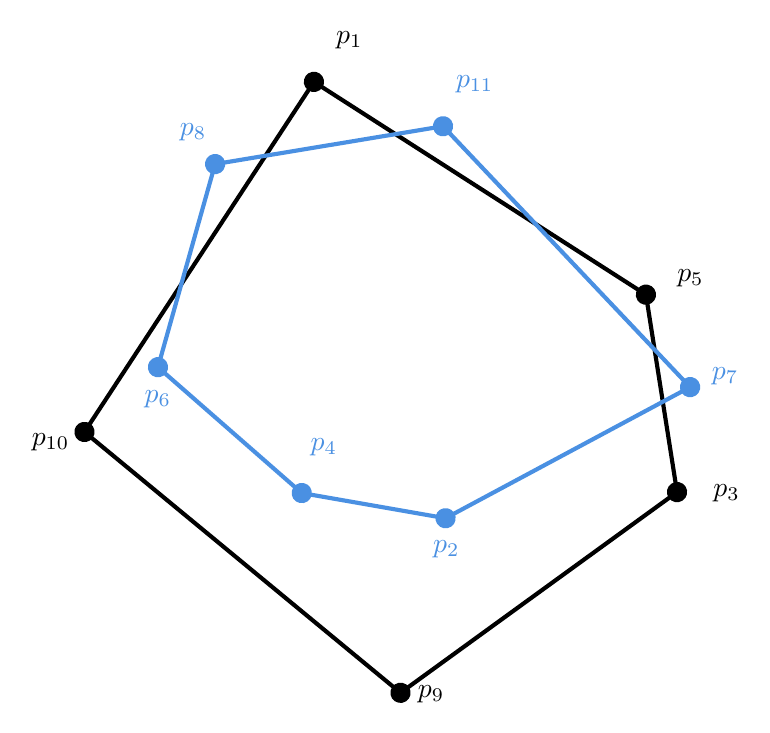
\begin{tikzpicture}[x=0.75pt,y=0.75pt,yscale=-1,xscale=1]
%uncomment if require: \path (0,391); %set diagram left start at 0, and has height of 391

%Flowchart: Connector [id:dp5289449572498183] 
\draw  [fill={rgb, 255:red, 0; green, 0; blue, 0 }  ,fill opacity=1 ] (239.33,364.26) .. controls (236.96,364.71) and (234.66,363.15) .. (234.21,360.78) .. controls (233.76,358.41) and (235.31,356.11) .. (237.69,355.66) .. controls (240.06,355.21) and (242.35,356.76) .. (242.81,359.14) .. controls (243.26,361.51) and (241.7,363.8) .. (239.33,364.26) -- cycle ;
%Flowchart: Connector [id:dp8854127292994846] 
\draw  [fill={rgb, 255:red, 0; green, 0; blue, 0 }  ,fill opacity=1 ] (87.06,238.59) .. controls (84.68,239.04) and (82.39,237.48) .. (81.94,235.11) .. controls (81.49,232.73) and (83.04,230.44) .. (85.42,229.99) .. controls (87.79,229.54) and (90.08,231.09) .. (90.54,233.47) .. controls (90.99,235.84) and (89.43,238.13) .. (87.06,238.59) -- cycle ;
%Flowchart: Connector [id:dp8118075796329792] 
\draw  [fill={rgb, 255:red, 0; green, 0; blue, 0 }  ,fill opacity=1 ] (357.58,172.44) .. controls (355.2,172.89) and (352.91,171.33) .. (352.46,168.96) .. controls (352,166.58) and (353.56,164.29) .. (355.94,163.84) .. controls (358.31,163.39) and (360.6,164.94) .. (361.05,167.32) .. controls (361.51,169.69) and (359.95,171.98) .. (357.58,172.44) -- cycle ;
%Flowchart: Connector [id:dp9423872091684253] 
\draw  [fill={rgb, 255:red, 0; green, 0; blue, 0 }  ,fill opacity=1 ] (372.56,267.55) .. controls (370.18,268.01) and (367.89,266.45) .. (367.44,264.08) .. controls (366.98,261.7) and (368.54,259.41) .. (370.92,258.96) .. controls (373.29,258.5) and (375.58,260.06) .. (376.04,262.43) .. controls (376.49,264.81) and (374.93,267.1) .. (372.56,267.55) -- cycle ;
%Flowchart: Connector [id:dp4355711900011987] 
\draw  [color={rgb, 255:red, 74; green, 144; blue, 226 }  ,draw opacity=1 ][fill={rgb, 255:red, 74; green, 144; blue, 226 }  ,fill opacity=1 ] (261.03,280.14) .. controls (258.66,280.59) and (256.37,279.04) .. (255.91,276.66) .. controls (255.46,274.29) and (257.02,272) .. (259.39,271.54) .. controls (261.77,271.09) and (264.06,272.65) .. (264.51,275.02) .. controls (264.96,277.39) and (263.41,279.69) .. (261.03,280.14) -- cycle ;
%Flowchart: Connector [id:dp42853879075832446] 
\draw  [fill={rgb, 255:red, 0; green, 0; blue, 0 }  ,fill opacity=1 ] (197.62,69.91) .. controls (195.25,70.36) and (192.95,68.8) .. (192.5,66.43) .. controls (192.05,64.05) and (193.6,61.76) .. (195.98,61.31) .. controls (198.35,60.85) and (200.64,62.41) .. (201.1,64.79) .. controls (201.55,67.16) and (199.99,69.45) .. (197.62,69.91) -- cycle ;
%Flowchart: Connector [id:dp9846986570623147] 
\draw  [color={rgb, 255:red, 74; green, 144; blue, 226 }  ,draw opacity=1 ][fill={rgb, 255:red, 74; green, 144; blue, 226 }  ,fill opacity=1 ] (122.47,207.37) .. controls (120.09,207.82) and (117.8,206.27) .. (117.35,203.89) .. controls (116.89,201.52) and (118.45,199.23) .. (120.83,198.77) .. controls (123.2,198.32) and (125.49,199.88) .. (125.94,202.25) .. controls (126.4,204.63) and (124.84,206.92) .. (122.47,207.37) -- cycle ;
%Straight Lines [id:da6555731265494601] 
\draw [color={rgb, 255:red, 0; green, 0; blue, 0 }  ,draw opacity=1 ][line width=1.5]    (371.74,263.26) -- (356.76,168.14) ;
%Straight Lines [id:da6904862039395101] 
\draw [color={rgb, 255:red, 0; green, 0; blue, 0 }  ,draw opacity=1 ][line width=1.5]    (238.51,359.96) -- (86.24,234.29) ;
%Straight Lines [id:da952195758093338] 
\draw [color={rgb, 255:red, 0; green, 0; blue, 0 }  ,draw opacity=1 ][fill={rgb, 255:red, 245; green, 166; blue, 35 }  ,fill opacity=1 ][line width=1.5]    (238.51,359.96) -- (298.38,316.5) -- (371.74,263.26) ;
%Straight Lines [id:da28876285645467437] 
\draw [color={rgb, 255:red, 0; green, 0; blue, 0 }  ,draw opacity=1 ][line width=1.5]    (86.24,234.29) -- (196.8,65.61) ;
%Straight Lines [id:da06843745010934266] 
\draw [color={rgb, 255:red, 0; green, 0; blue, 0 }  ,draw opacity=1 ][line width=1.5]    (356.76,168.14) -- (196.8,65.61) ;
%Flowchart: Connector [id:dp8647675221499903] 
\draw  [color={rgb, 255:red, 74; green, 144; blue, 226 }  ,draw opacity=1 ][fill={rgb, 255:red, 74; green, 144; blue, 226 }  ,fill opacity=1 ] (191.75,268.01) .. controls (189.38,268.47) and (187.08,266.91) .. (186.63,264.54) .. controls (186.18,262.16) and (187.73,259.87) .. (190.11,259.42) .. controls (192.48,258.96) and (194.77,260.52) .. (195.23,262.89) .. controls (195.68,265.27) and (194.12,267.56) .. (191.75,268.01) -- cycle ;
%Flowchart: Connector [id:dp8591737152826057] 
\draw  [color={rgb, 255:red, 74; green, 144; blue, 226 }  ,draw opacity=1 ][fill={rgb, 255:red, 74; green, 144; blue, 226 }  ,fill opacity=1 ] (378.85,216.97) .. controls (376.48,217.43) and (374.18,215.87) .. (373.73,213.5) .. controls (373.28,211.12) and (374.83,208.83) .. (377.21,208.38) .. controls (379.58,207.92) and (381.87,209.48) .. (382.33,211.86) .. controls (382.78,214.23) and (381.22,216.52) .. (378.85,216.97) -- cycle ;
%Flowchart: Connector [id:dp24142143741497757] 
\draw  [color={rgb, 255:red, 74; green, 144; blue, 226 }  ,draw opacity=1 ][fill={rgb, 255:red, 74; green, 144; blue, 226 }  ,fill opacity=1 ] (259.82,91.3) .. controls (257.45,91.75) and (255.15,90.19) .. (254.7,87.82) .. controls (254.25,85.45) and (255.81,83.15) .. (258.18,82.7) .. controls (260.55,82.25) and (262.85,83.81) .. (263.3,86.18) .. controls (263.75,88.55) and (262.19,90.85) .. (259.82,91.3) -- cycle ;
%Flowchart: Connector [id:dp8761002853248444] 
\draw  [color={rgb, 255:red, 74; green, 144; blue, 226 }  ,draw opacity=1 ][fill={rgb, 255:red, 74; green, 144; blue, 226 }  ,fill opacity=1 ] (150.01,109.52) .. controls (147.64,109.97) and (145.35,108.41) .. (144.89,106.04) .. controls (144.44,103.67) and (146,101.37) .. (148.37,100.92) .. controls (150.75,100.47) and (153.04,102.02) .. (153.49,104.4) .. controls (153.95,106.77) and (152.39,109.06) .. (150.01,109.52) -- cycle ;
%Straight Lines [id:da9084013306880081] 
\draw [color={rgb, 255:red, 74; green, 144; blue, 226 }  ,draw opacity=1 ][line width=1.5]    (190.93,263.72) -- (121.65,203.07) ;
%Straight Lines [id:da1404095072194267] 
\draw [color={rgb, 255:red, 74; green, 144; blue, 226 }  ,draw opacity=1 ][line width=1.5]    (260.21,275.84) -- (190.93,263.72) ;
%Straight Lines [id:da6896268175375341] 
\draw [color={rgb, 255:red, 74; green, 144; blue, 226 }  ,draw opacity=1 ][line width=1.5]    (378.03,212.68) -- (259,87) ;
%Straight Lines [id:da7446132704342231] 
\draw [color={rgb, 255:red, 74; green, 144; blue, 226 }  ,draw opacity=1 ][line width=1.5]    (259,87) -- (149.19,105.22) ;
%Straight Lines [id:da9602389416745392] 
\draw [color={rgb, 255:red, 74; green, 144; blue, 226 }  ,draw opacity=1 ][line width=1.5]    (378.03,212.68) -- (260.21,275.84) ;
%Straight Lines [id:da5460434431084907] 
\draw [color={rgb, 255:red, 74; green, 144; blue, 226 }  ,draw opacity=1 ][line width=1.5]    (149.19,105.22) -- (121.65,203.07) ;

% Text Node
\draw (206,40) node [anchor=north west][inner sep=0.75pt]   [align=left] {$\displaystyle p_{1}$};
% Text Node
\draw (252.75,285) node [anchor=north west][inner sep=0.75pt]  [color={rgb, 255:red, 74; green, 144; blue, 226 }  ,opacity=1 ] [align=left] {$\displaystyle p_{2}$};
% Text Node
\draw (193.75,236) node [anchor=north west][inner sep=0.75pt]  [color={rgb, 255:red, 74; green, 144; blue, 226 }  ,opacity=1 ] [align=left] {$\displaystyle p_{4}$};
% Text Node
\draw (113.75,213) node [anchor=north west][inner sep=0.75pt]  [color={rgb, 255:red, 74; green, 144; blue, 226 }  ,opacity=1 ] [align=left] {$\displaystyle p_{6}$};
% Text Node
\draw (387.03,201.68) node [anchor=north west][inner sep=0.75pt]  [color={rgb, 255:red, 74; green, 144; blue, 226 }  ,opacity=1 ] [align=left] {$\displaystyle p_{7}$};
% Text Node
\draw (387.75,258) node [anchor=north west][inner sep=0.75pt]   [align=left] {$\displaystyle p_{3}$};
% Text Node
\draw (245.38,354.75) node [anchor=north west][inner sep=0.75pt]   [align=left] {$\displaystyle p_{9}$};
% Text Node
\draw (59.38,233.38) node [anchor=north west][inner sep=0.75pt]   [align=left] {$\displaystyle p_{10}$};
% Text Node
\draw (370.38,154.38) node [anchor=north west][inner sep=0.75pt]   [align=left] {$\displaystyle p_{5}$};
% Text Node
\draw (130.75,84) node [anchor=north west][inner sep=0.75pt]  [color={rgb, 255:red, 74; green, 144; blue, 226 }  ,opacity=1 ] [align=left] {$\displaystyle p_{8}$};
% Text Node
\draw (263.75,61) node [anchor=north west][inner sep=0.75pt]  [color={rgb, 255:red, 74; green, 144; blue, 226 }  ,opacity=1 ] [align=left] {$\displaystyle p_{11}$};


\end{tikzpicture}

